\section{Projectactiviteiten}

SUNRISE is onderverdeeld in 3 delen: 

\begin{itemize}
\item Er moet een website en app gemaakt worden.
\item Het systeem in de fietsenstalling moet bestuurd worden door een minicomputer (ODROID).
\item De verbinding tussen de website en de minicomputer moet gaan via een server. De server houdt middels een database alle data bij over de gebruiker en het systeem.


\end{itemize}
%Er moet een website en app gemaakt worden. Het systeem in de fietsen stalling word %bestuurd door een minicomputer(ODRIOD). De verbinding tussen de website en de mini %computer moet gaan via een server. De server houd ook alle data bij over de %gebruiker en het systeem.
\noindent
Het team is opgedeeld in 3 groepen van 2 personen.\\

\subsection{Groep IO}
De website wordt gemaakt door middel van HTML5 en Canvas. Daarnaast moet er ook een app gemaakt worden. Hierin moet de gebruiker kunnen inloggen, registreren en de fietsenstalling bedienen. De website bestaat uit een deel met informatie voor de media en een deel voor de uiteindelijke gebruikers.

\subsection{Groep Server}
De server wordt gemaakt door middel van PHP. Hierbij moet er ook een website gemaakt worden voor de systeem administrator. Op deze website is alle data van het systeem af te lezen, zoals de status van de accu's en zonnepanelen. Aan de server zit een SQL server verbonden waarin alle data wordt opgeslagen. Daarnaast moet deze groep de connectie verzorgen tussen de ODROID en de server met behulp van C-code.

\subsection{Groep ODROID}
Deze groep zorgt voor het verwerken van de data van het weerstation en de Victron. Dit wordt gedaan door middel van het Modbus protocol en C-code. Daarnaast moet de ODROID bijhouden hoelang de fiets nog moet opladen. Als de gebruiker inlogt en een stopcontact reserveert moet de ODROID er voor zorgen dat er spanning komt te staan op het stopcontact.\\

\noindent
Figuur \ref{fig:overview} geeft een overzicht van alle projectactiviteiten.

\begin{figure}[htbp]
\centering
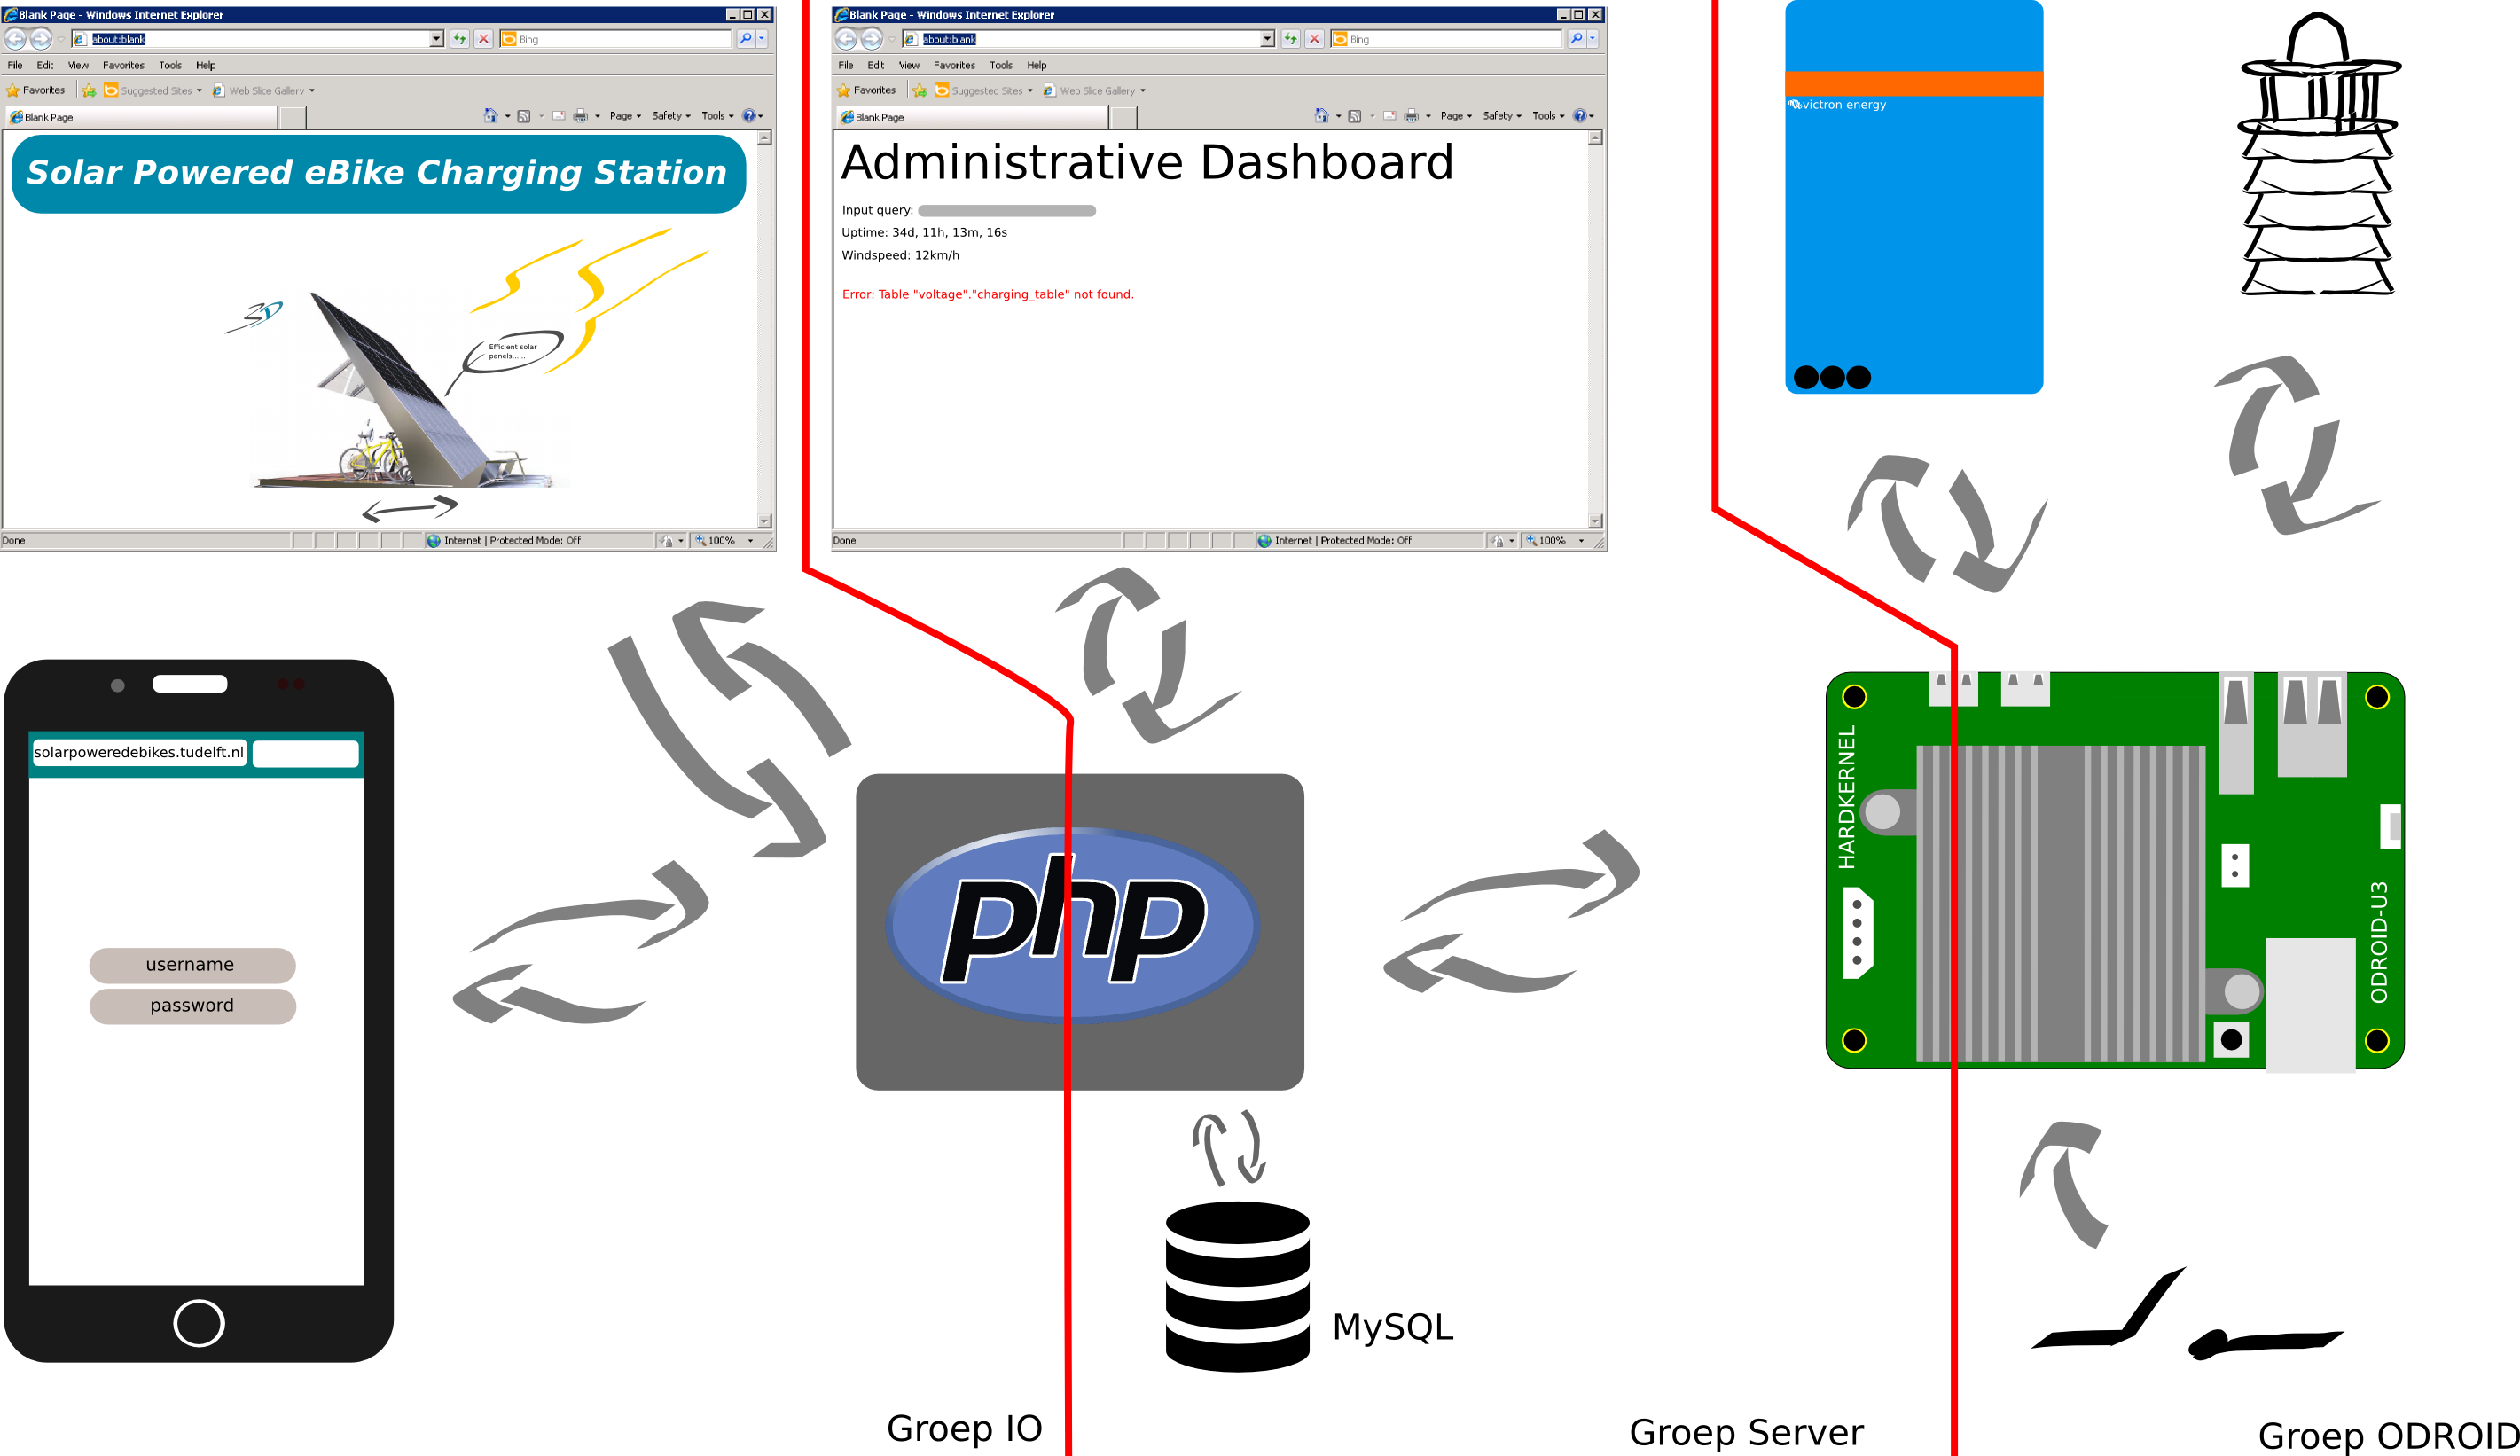
\includegraphics[width=1.1\textwidth]{project_overview.png}
\caption{Projectactiviteiten voor Project SUNRISE}\label{fig:overview}
\end{figure}